% !TEX root=./report.tex

\section{Approach}
In this paper we propose two algorithms to solve distinct problems that arise from real-world disturbances that act upon the ITS.

\subsection{Dynamic Stabilization}
\label{sec:dynamic_stabilization_approach}

\begin{figure}[t]
   \begin{center}
      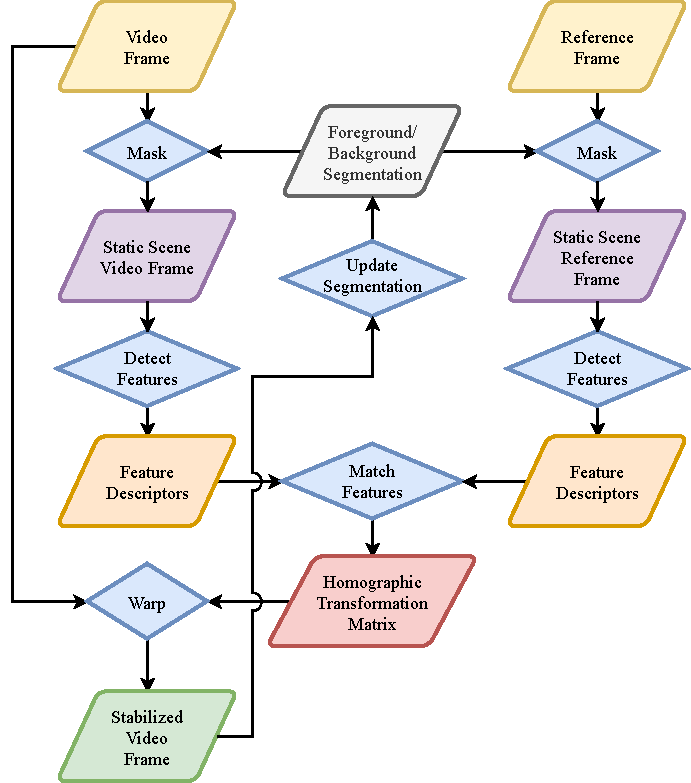
\includegraphics[width=0.8\linewidth]{diagrams/DynamicStabilization.pdf}
   \end{center}
   \caption{
      The proposed dynamic stabilization pipeline. 
      The input is the video and a stable reference frame.
      The frames are segmented into the foreground and background to extract the static scene.
      On the static scene visual features are detected and the feature descriptors are matched.
      We use the homographic transformation minimizing the reprojection-error based on the matching to warp the video frame.
      The stabilized frame is used to update the background segmentation mask.
       }
   \label{fig:dynamic_stabilization_algorithm}
\end{figure}

The camera sensors used in the project are mounted to gantry bridges spanning over the highway.
Environmental influences, \eg{} wind or vibrations from passing vehicles, bring the bridges into a swinging state that spreads onto the cameras. 
This unwanted real world movement propagates into the video feeds output by the cameras and introduces jittery motion in image space. 
We assume the cameras to be mostly static, thus we only face disturbances within a small range around the resting position.
Nonetheless, the small disturbances get amplified by the huge distances covered by the cameras and introduce substantial error.

To mitigate the noise added by the jittery motion we propose the pipeline displayed in \Cref{fig:dynamic_stabilization_algorithm} and explained in the following.

%%%%%%%%%%%%%%%%%%%%%%%%%%%%%%%%%%%%%%%%%%%%%%%%%%%%%%%%%%%%%%%%%%%%%%%%%%%%%%%%%%%%%%%%%%%%%%%%%%%%%%%%%%%%%%%%%%%%
%%%%%%%%%%%%%%%%%%%%%%%%%%%%%%%%%%%%%%%%%%%%%%%%%%%%%%%%%%%%%%%%%%%%%%%%%%%%%%%%%%%%%%%%%%%%%%%%%%%%%%%%%%%%%%%%%%%%
%%%%%%%%%%%%%%%%%%%%%%%%%%%%%%%%%%%%%%%%%%%%%%%%%%%%%%%%%%%%%%%%%%%%%%%%%%%%%%%%%%%%%%%%%%%%%%%%%%%%%%%%%%%%%%%%%%%%

\paragraph{Extract Static Background}
We stabilize the input frame by minimizing the reprojection-error between the video frame and the reference frame, thus aligning the images.
This alignment is based on the matching of features between the frames, whereas we do not align the moving vehicles, but only the static non-moving background, \eg{} the road, poles, guardrails and bridges.
We assume that the background does not move in the real world, thus aligning it during image warping ensures that the scene stays static and only the vehicles real movement is kept.
Hence, we extract the static background from the input frame and the stable reference frame using a background segmentation based on
the \emph{Improved Adaptive Gaussian Mixture Model for Background Subtraction} proposed by Zoran Zivkovic \etal{} \cite{zivkovic10.5555/1018428.1020644,zivkovic10.1016/j.patrec.2005.11.005,opencv_library}.

%%%%%%%%%%%%%%%%%%%%%%%%%%%%%%%%%%%%%%%%%%%%%%%%%%%%%%%%%%%%%%%%%%%%%%%%%%%%%%%%%%%%%%%%%%%%%%%%%%%%%%%%%%%%%%%%%%%%
%%%%%%%%%%%%%%%%%%%%%%%%%%%%%%%%%%%%%%%%%%%%%%%%%%%%%%%%%%%%%%%%%%%%%%%%%%%%%%%%%%%%%%%%%%%%%%%%%%%%%%%%%%%%%%%%%%%%
%%%%%%%%%%%%%%%%%%%%%%%%%%%%%%%%%%%%%%%%%%%%%%%%%%%%%%%%%%%%%%%%%%%%%%%%%%%%%%%%%%%%%%%%%%%%%%%%%%%%%%%%%%%%%%%%%%%%

\paragraph{Feature Detection}
\begin{figure}[t]
   \begin{center}
      \includegraphics[width=\linewidth]{images/feature_matching.png}
   \end{center}
   \caption{
      Left: The input frame. 
      Right: The stable reference frame.
      The colorful lines display the matching between image features. 
      The ends of the lines are the location of the features.
       }
   \label{fig:dynamic_stabilization_feature_matching}
\end{figure}

We search the static background for pixel locations that are prominent and depict specific patterns that are unique and can easily be compared.
The detected features describe the location based on different metrics, \eg{} the local image gradient, oriented histograms or haar-like features \cite{stork2001pattern}.
Kumar \etal{} \cite{kumar2014survey} give in depth descriptions of a multitude of feature detectors and descriptors.

We implemented the SURF \cite{bay10.1007/11744023_32} and ORB \cite{rublee6126544} feature detectors and descriptors and the Fast \cite{Ghahremani_2021} feature detector with FREAK \cite{alahi6247715} feature descriptors. The algorithmic implementation is included in the OpenCV library \cite{opencv_library}. 

%%%%%%%%%%%%%%%%%%%%%%%%%%%%%%%%%%%%%%%%%%%%%%%%%%%%%%%%%%%%%%%%%%%%%%%%%%%%%%%%%%%%%%%%%%%%%%%%%%%%%%%%%%%%%%%%%%%%
%%%%%%%%%%%%%%%%%%%%%%%%%%%%%%%%%%%%%%%%%%%%%%%%%%%%%%%%%%%%%%%%%%%%%%%%%%%%%%%%%%%%%%%%%%%%%%%%%%%%%%%%%%%%%%%%%%%%
%%%%%%%%%%%%%%%%%%%%%%%%%%%%%%%%%%%%%%%%%%%%%%%%%%%%%%%%%%%%%%%%%%%%%%%%%%%%%%%%%%%%%%%%%%%%%%%%%%%%%%%%%%%%%%%%%%%%

\paragraph{Feature Matching}
We compare the detected features from the input frame with the features from the stable reference frame.
A match is reported if the feature descriptors of two compared features surpass the Lowe's ratio test \cite{lowe10.1023/B:VISI.0000029664.99615.94} regarding some feature dependent metric \cite{kumar2014survey}.
These feature matches establish a spatial relationship in pixel space between the two frames.
\Cref{fig:dynamic_stabilization_feature_matching} displays an exemplary feature matching.

We estimate a homographic transformation $H$ that maps the homogeneous pixel locations $(x_i, y_i, 1)^T$ of the input frame to the matched pixel locations $(x'_i, y'_i, 1)^T$ in the stable reference frame.
We minimize the reprojection-error between the pixels so that for each match $i$ it holds
\begin{equation}
 z_i  * (x'_i, y'_i, 1)^T \sim H * (x_i, y_i, 1)^T
 \label{eq:dynamic_stabilization_homographic_transformation}
\end{equation}
where $z_i$ is the homogeneous component used in the perspective division. 
We use a RANSAC \cite{fischler1981random} based estimation procedure to robustify the minimization against outliers.

The algorithmic implementation is included in the OpenCV library \cite{opencv_library}.

%%%%%%%%%%%%%%%%%%%%%%%%%%%%%%%%%%%%%%%%%%%%%%%%%%%%%%%%%%%%%%%%%%%%%%%%%%%%%%%%%%%%%%%%%%%%%%%%%%%%%%%%%%%%%%%%%%%%
%%%%%%%%%%%%%%%%%%%%%%%%%%%%%%%%%%%%%%%%%%%%%%%%%%%%%%%%%%%%%%%%%%%%%%%%%%%%%%%%%%%%%%%%%%%%%%%%%%%%%%%%%%%%%%%%%%%%
%%%%%%%%%%%%%%%%%%%%%%%%%%%%%%%%%%%%%%%%%%%%%%%%%%%%%%%%%%%%%%%%%%%%%%%%%%%%%%%%%%%%%%%%%%%%%%%%%%%%%%%%%%%%%%%%%%%%

\paragraph{Image Alignment}
We use the found homographic transformation to warp the whole input frame, thus aligning the background of the frames.
As the keyframe is stable and does not change over time the current video frame is also stabilized.
The alignment minimizes the motion of the static background scene and leaves only the real expected movement of the vehicles.

%%%%%%%%%%%%%%%%%%%%%%%%%%%%%%%%%%%%%%%%%%%%%%%%%%%%%%%%%%%%%%%%%%%%%%%%%%%%%%%%%%%%%%%%%%%%%%%%%%%%%%%%%%%%%%%%%%%%
%%%%%%%%%%%%%%%%%%%%%%%%%%%%%%%%%%%%%%%%%%%%%%%%%%%%%%%%%%%%%%%%%%%%%%%%%%%%%%%%%%%%%%%%%%%%%%%%%%%%%%%%%%%%%%%%%%%%
%%%%%%%%%%%%%%%%%%%%%%%%%%%%%%%%%%%%%%%%%%%%%%%%%%%%%%%%%%%%%%%%%%%%%%%%%%%%%%%%%%%%%%%%%%%%%%%%%%%%%%%%%%%%%%%%%%%%

\paragraph{Upate of Background Segmentation}
We use the stabilized frame to update the segmentation of the foreground and background.
We assume the motion between frames to be relatively small, thus we use the segmentation of the stabilized frame for the next frame.
This reduces the search space for the feature detectors and prohibits matches between static scene and dynamic foreground objects. 
% Hence, the algorithm is robustified and speed up.
